Dette er fagrapporten til Team 4 i Eksperter i Team, VR-Landsbyen. Den beskriver det faglige produktet som ble utviklet i l�pet av semesteret. Produktet er en l�sning for virtuell virkelighet, og denne rapporten inneholder hva gruppen fant ut i l�pet av en forstudie, kravspesifikasjonen til l�sningen sammen med beskrivelse design og implementasjon og til slutt en presentasjon av resultatet av prosjektet.

\section{Problemstilling}

	Hvordan f� lagd en rimelig og brukbar prototyp for tracking av hode til bruk i VR.

	\begin{itemize}
		\item Lav kostnad i forhold til lignende brukter p� markedet i dag
		\item Enkelt oppsett og brukevennlig
	\end{itemize}
	
	Oppgaven som gruppa valgte var Inexpensive Tracked VR. Dette var fordi gruppa synes denne oppgaven hadde h�yeste wow faktor, og fordi gruppa f�lte at kompentansen for � l�se den var tilstede. Gruppa ble enige om � bruke et headset til � feste IR dioder p�, og s� tracke dem ved hjelp av et hd kamera for � kunne st� et stykke unna skjermen.

\section{Ressurser}

	Dette er krevende prosjekt som trenger personer med gode faglige og teknologiske kunnskaper innen data, elektronikk og petroleum. Og med personer i gruppa innefor alle disse faglige feltene ble prosjektet gjennomf�rbart. Vi fikk ogs� mye hjelp fra ressurssterke personer utenfor gruppa innen data og elektronikk og vi fikk god hjelp fra Omega-verksted og IPT verkstedet.
	
	Dette prosjektet er ganske omfattende og kostnadskrevende med innkj�p av dyrt elektronisk utstyr. Derfor er samarbeidet og den �konomiske st�tten fra StatoilHydro sv�rt viktig. Det er blitt gjort mye innkj�p av utstyr i forbindelse med prosjektet selv om ikke alt er brukt i v�r endelige prototyp. Institutt for Petroleumsteknologi har gitt oss tilgjenglighet til mye avansert datautstyr som har v�rt viktig for gjennomf�relsen av prosjektet.
	
\section{Teamet}

	Vi best�r av 5 studenter p� NTNU. To g�r siv.ing. datateknikk, en g�r siv.ing. elektronikk, en g�r siv.ing. petroleumsteknologi og en g�r medisin. Vi er fire stykker fra 4. klasse og en fra 5., og alderen er fra 22 til 24 �r.

	\begin{figure}[h]
	\centering
	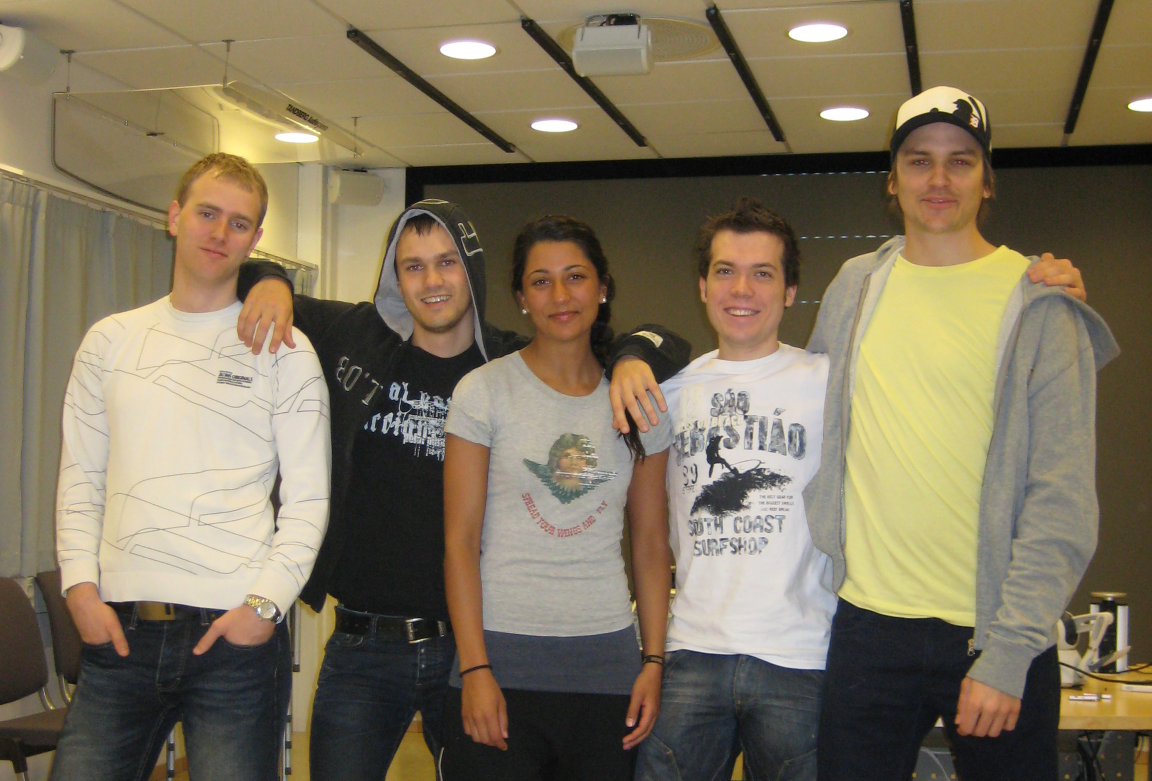
\includegraphics[width=0.60\textwidth]{graphics/people.png}
	\caption{Team 4. (Fra venstre) Jon Skarpetveit, Vegar Neshaug, Rahele Zarabi, Holger Ludvigsen, Kristoffer Selboe}
	\label{fig:people}
	\end{figure}